\chapter{Firewall Avanzati}

Applicazioni come Telnet, SSH, rlogin \dots sono semplici da gestire con 
packet filtering, perché per loro natura implicano ruoli ben definiti: client 
e server; il pattern di scambio è un semplice request/reply.

Altre applicazioni possono avere protocolli più elaborati; quando lo 
scambio a livello di trasporto diventa più articolato, gestire il firewall 
diventa più complesso:
\begin{itemize}
    \item studiare molto bene i protocolli applicativi 
    \item verificare debolezze del filtraggio 
    \item essere consapevoli di cosa non si riesce a fare con il filtraggio 
\end{itemize}

\section{Packet Filtering Avanzati}

\subsection{SMTP (Simple Mail Transfer Protocol)}
Gestisce lo scambio di messaggi di posta elettronica:
\begin{itemize}
    \item la connessione tra i diversi server di posta avviene attraverso una connessione 
    TCP (porta 25)
    \item Ogni utente è identificato dall'indirizzo \textit{nomeutente@indirizzo\_server}
\end{itemize}

\noindent Il client a livello utente utilizza SMTP solo per inviare il messaggio al 
server mail, il quale poi lo invierà \textit{"davvero"}.

\subsubsection{I comandi}
I principali comandi SMTP:
\begin{itemize}
    \item \textbf{HELO}: identifica il client SMTP al server SMTP
    \item \textbf{EHLO}: possibile usare anche questo comando per identificarsi, se supportato dal server
    \item \textbf{MAIL FROM $<$indirizzo mittente$>$}: indica mailbox del mittente 
    \item \textbf{RCPT TO $<$indirizzo destinatario$>$}: mailbox destinatario; è possibile 
    indicare molteplici destinatari 
    \item \textbf{DATA}: indica al server che quanto digitato successivamente sono i dati del messaggio di posta
    \item \textbf{RSET}: annulla i comandi precedentemente inviati nella sessione corrente 
    \item \textbf{VRFY $<$stringa$>$}: chiede al server se la stringa rappresenta un nome utente, ed in tal 
    caso visualizza il suo indirizzo 
    \item \textbf{HELP}: visualizza i comandi disponibili sul server 
    \item \textbf{NOOP}: non esegue alcuna operazione, restituisce un messaggio 250 (OK) se il server risponde 
    \item \textbf{QUIT}: termina la sessione corrente
\end{itemize}

\subsubsection{Le fasi}
Una sessione SMTP attraversa almeno sei fasi:
\begin{enumerate}
    \item Il client SMTP contatta il server sulla porta 25; se è in ascolto e 
    la connessione è accettata risponde con un messaggio 220 (\textit{Ready})
    \item Il client chiede di stabilire la connessione inviando il comando HELO seguito 
    dal FQDN (Fully Qualified Domain Name); se il server accetta risponde con 250 (OK)
    \item Il client indica il proprio indirizzo tramite il comando MAIL FROM; il server risponde 250 (OK)
    \item Il client indica i destinatari tramite RCPT TO; il server risponde 250 (OK) per ogni destinatario accettato 
    \item Il client comunica l'intenzione di scrivere il corpo del messaggio con DATA
    \item Completato il messaggio il server memorizza la mail; è possibile scrivere un nuovo messaggio 
    oppure inviare il comando QUIT, dopo il quale il server invia i messaggi e risponde con Closing (221); la 
    connessione TCP viene terminata
\end{enumerate}

\subsubsection{I codici di risposta}
Il server risponde ad ogni comando con un codice di tre cifre che ha la 
seguente interpretazione:
\begin{itemize}
    \item 1xx: messaggio informativo
    \item 2xx: comando eseguito e terminato con successo 
    \item 3xx: comando eseguito e terminato con successo che richiede di essere 
    seguito da altri comandi 
    \item 4xx: errore temporaneo nell'esecuzione del comando, ma il dialogo non è compromesso 
    \item 5xx: errore grave, il dialogo è compromesso e dovrà essere ripreso dall'inizio
\end{itemize}

\subsubsection{Protezione}
\begin{itemize}
    \item Protezione anti-spam minimale
    \begin{itemize}
        \item verifica del dominio del mittente 
        \item login obbligatorio
        
        $\rightarrow$ fatto per evitare \textbf{\textit{open relay}}, ovvero la capacità di mandare posta 
        senza essere autenticato 
    \end{itemize}
    \item Si aggiunge la criptazione al servizio di posta (con SSL/TLS); così viene criptata 
    il \textit{canale} ma non il messaggio, quindi un server intermediario può leggere 

    $\rightarrow$ se voglio criptare anche il messaggio si usa un altro protocollo (PGP)
\end{itemize}

\subsubsection{Packet Filtering}
\begin{itemize}
    \item \textbf{Politica:} nella rete aziendale un solo server SMTP è autorizzato 
    a gestire la posta elettronica con l'esterno 
    
    $\rightarrow$ bisogna gestire due connessioni TCP:
    \begin{itemize}
        \item Ricevere posta elettronica: altri mail server si connettono al mail server aziendale agendo da client 
        \item Inviare posta elettronica: il mail server aziendale si connette ad altri mail server agendo da client
    \end{itemize}
\end{itemize}

\begin{figure}[H]
    \centering
    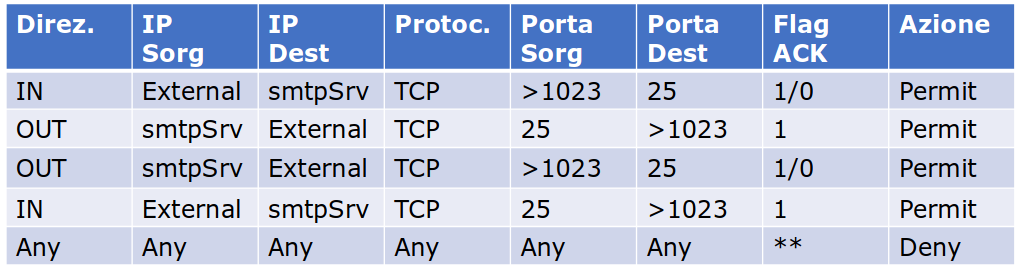
\includegraphics[width=1\linewidth]{chapters/12/images/smtp.png}
\end{figure}

\subsection{FTP (File Transfer Protocol)}
FTP è il protocollo generalmente usato per trasferire dati tra due host, con l'obiettivo 
di farlo in maniera efficiente ed affidabile; per questo motivo si basa su TCP (porta 21).

\noindent FTP utilizza due processi distinti:
\begin{itemize}
    \item \textit{Protocol Interpreter} (PI) attraverso cui il client invia comandi e riceve le risposte del server 
    \item \textit{Data Transfer Process} (DTP) attraverso cui il client ed il server si scambiano dati;
    può essere di due tipi:
    \begin{itemize}
        \item Attivo: il client contatta il server il quale da inizio alla connessione 
        \item Passivo: è prerorgativa del client anche dare il via alla connessione
    \end{itemize}
\end{itemize}

\subsubsection{Le fasi}
\begin{enumerate}
    \item Il client contatta il server sulla porta 21 usando il PI
    \item Autenticazione del client 
    \item Trasferimento dati tramite DTP 
    \item Termine della sessione TCP 
\end{enumerate}

\subsubsection{Connessioni FTP}
Ci sono due connessioni TCP per ogni sessione FTP:
\begin{itemize}
    \item \textbf{Connessione di controllo:} usata dal client per inviare i comandi e 
    dal server per comunicare i codici di risposta; viene aperta dal client che si connette 
    al server sulla porta TCP 21 
    \item \textbf{Connessione dati:} usata per il trasferimento dei file, viene aperta 
    dal server sulla porta 20
\end{itemize} 

\noindent La connessione dati viene aperta dal server verso il client:
\begin{center}
    \texttt{ftpServer:20} $\rightarrow$ \texttt{ftpClient:XXXX}
\end{center}

\noindent dove XXXX è la porta definita dinamicamente dal client.

\noindent $\rightarrow$ Non è possibile applicare la solita politica di gestione, dato che 
la connessione da esterno ad interno è obbligata ma non sappiamo a priori la porta.

\noindent Rischio:
\begin{center}
    \texttt{Intusore:20} $\rightarrow$ \texttt{Vittima:XXXX}
\end{center}

\noindent Le porte $>$1023 sono usate da servizi molto diffusi e da trojan.

\begin{figure}[H]
    \centering
    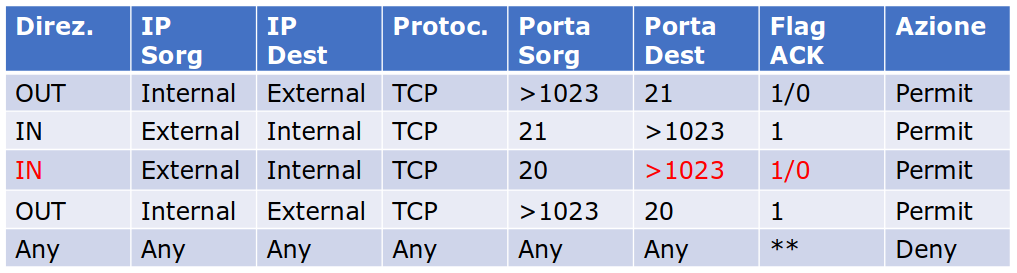
\includegraphics[width=1\linewidth]{chapters/12/images/ftp1.png}
\end{figure}

\noindent Dovrei usare un packet filtering che si ricordi delle connessioni.
\subsubsection{Soluzione}
La connessione dati viene aperta dal client verso il server (DTP passivo).

\begin{center}
    \texttt{ftpClient:YYYY} $\rightarrow$ \texttt{ftpServer:XXXX}
\end{center}

La politica di gestione \textit{connessioni solo da interno ad esterno} torna 
ad essere applicabile. Ora tutti gli FTP supportano la modalità passiva di default.

\begin{figure}[H]
    \centering
    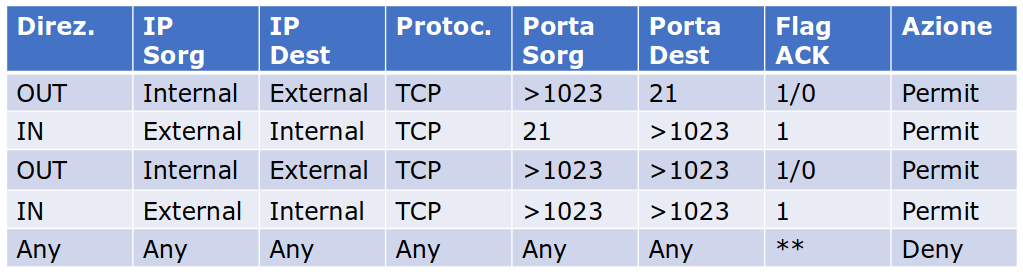
\includegraphics[width=1\linewidth]{chapters/12/images/ftp2.png}
\end{figure}

\subsection{Attacco RPC}
Remote Call Procedure è un protocollo che può essere utilizzato 
da un'applicazione per richiedere un serivizio a un programma residente su un 
altro computer in rete. 
\noindent È stata riscontrata una vulnerabilità che potrebbe portare all'esecuzione 
di codice non autorizzato.

\noindent A livello di firewall il problema è che non si conosce a priori la
porta che il server RPC assegnerà al servizio. Rischio:
\begin{center}
    \texttt{Intrusore:YYYY} $\rightarrow$ \texttt{ServerRPC-Vittima:XXXX}
\end{center}

\section{New Generation Packet Filtering}

Lo svantaggio principale dell'approccio SPF risiede nell'\textbf{array di porte 
che devono essere lasciate aperte} per tutto il tempo per permettere il 
traffico desiderato.

\subsubsection{Dynamic Packet Filter}

\noindent Per superare questo problema sono stati sviluppati dei \textbf{Dynamic Packet Filter},
che aprono e chiudono le porte sul firewall in base alle info dell'header dei 
pacchetti che transitano attraverso di essi; una volta che una serie di pacchetti 
ha transitato attraverso la porta, il firewall richiude la porta.

\subsubsection{Stateful Packet Filter}
È una evoluzione del dynamic ma \textit{state-aware}:
\begin{itemize}
    \item prende informazioni dai livelli superiori (trasporto e/o applicativo) per cercare di adattare 
    di conseguenza le regole di filtraggio 
    \item distingue le nuove connessioni da quelle già apert, tenendo traccia delle sessioni
\end{itemize}

\subsection{Vantaggi e Svantaggi del Dynamic Packet Filter}
\begin{itemize}
    \item \textbf{\textcolor{darkgreen}{Vantaggi:}}
    \begin{itemize}
        \item le porte sono aperte solo temporaneamente sul perimetro della rete 
        \item supporta quasi tutti i servizi 
        \item molti attacchi che funzionano su SPF sono difficili o impossibili da replicare 
        su DPF
    \end{itemize}
    \item \textbf{\textcolor{red}{Svantaggi:}}
    \begin{itemize}
        \item permettono connessioni IP dirette verso gli host interni della rete
        \item non garantiscono alcuna autenticazione
        \item soggetto ad attacchi che mirano alla saturazione della tabella  
    \end{itemize}
\end{itemize}

\subsection{Connessioni TCP - stateful firewall}
\begin{itemize}
    \item Alla ricezioni di un SYN $\rightarrow$ verifica dell'ACL
    \begin{itemize}
        \item connessione non autorizzata $\rightarrow$ deny 
        \item connessione autorizzata $\rightarrow$ accept e scrittura di una entry nella connection table 
    \end{itemize}
    \item Ricezione di pacchetti successivi $\rightarrow$ verifica della connection table
\end{itemize}

\noindent $\rightarrow$ è necessario definire solo le regole relative all'apertura delle 
connessioni TCP (pacchetto SYN)

\subsection{UDP - stateful firewall}
UDP non ha uno stato della connessione per definizione; viene impostato dunque un \textbf{timeout}
verificando anche chi ha impostato la connessione per primo.
\noindent Molti sistemi stateful hanno la possibilità di fare filtraggio applicativo:
\begin{itemize}
    \item comporta che il firewall faccia il parsing del pacchetto e conosca i protocolli 
    \item tutto ciò a scapito delle performance
\end{itemize}

\subsection{Deep Packet Inspection}
Il controllo non viene fatto solo sul protocollo ma anche sul pattern di comunicazione usato. Ad 
esempio, le richieste che rispettano il protocollo ma sono tipicamente usate per un attacco vengono respinte.
\begin{itemize}
    \item offre una protezione migliore
    \item definizione più semplice della politica 
    \item impatta pesantemente sulle prestazioni
\end{itemize}



